\documentclass{article}
\usepackage{mirex2010,amsmath,cite}
\usepackage{graphicx}
\usepackage{tikz}
\usetikzlibrary{arrows,positioning}

% Defines a `datastore' shape for use in DFDs.  This inherits from a
% rectangle and only draws two horizontal lines.
\makeatletter
\pgfdeclareshape{datastore}{
  \inheritsavedanchors[from=rectangle]
  \inheritanchorborder[from=rectangle]
  \inheritanchor[from=rectangle]{center}
  \inheritanchor[from=rectangle]{base}
  \inheritanchor[from=rectangle]{north}
  \inheritanchor[from=rectangle]{north east}
  \inheritanchor[from=rectangle]{east}
  \inheritanchor[from=rectangle]{south east}
  \inheritanchor[from=rectangle]{south}
  \inheritanchor[from=rectangle]{south west}
  \inheritanchor[from=rectangle]{west}
  \inheritanchor[from=rectangle]{north west}
  \backgroundpath{
    %  store lower right in xa/ya and upper right in xb/yb
    \southwest \pgf@xa=\pgf@x \pgf@ya=\pgf@y
    \northeast \pgf@xb=\pgf@x \pgf@yb=\pgf@y
    \pgfpathmoveto{\pgfpoint{\pgf@xa}{\pgf@ya}}
    \pgfpathlineto{\pgfpoint{\pgf@xb}{\pgf@ya}}
    \pgfpathmoveto{\pgfpoint{\pgf@xa}{\pgf@yb}}
    \pgfpathlineto{\pgfpoint{\pgf@xb}{\pgf@yb}}
 }
}
\makeatother



% Title.
% ------
\title{Audio Classical Composer Identification in MIREX 2015: submission based on structural analysis of music}

% Single address
\oneauthor
  {Leopoldo Pla Sempere} {Polytechnic University of Valencia \\ {\tt leoplsem@posgrado.upv.es}}

\begin{document}
%
\maketitle
%
\begin{abstract}
Based on musicological fundamentals of classical composers and the structural analysis primary ideas, in this work I study some compositive features to train a neural network using author recognition techniques applied to the task of Audio Classical Composer Identification in MIREX 2015. 
\end{abstract}
%


\section{Introduction}\label{sec:introduction}

I propose a model based on some of the high level features that the humans use to identify a composer in an audio or a score: musical structure and harmonic analysis.  These features are parallel to the features that is usual to look for in a text, as POS tagging, n-grams, different kind of element counts (number of punctuation marks, hyphens, number of paragraphs, etc.) or the general structure of the text (introduction, development of the text, conclusion, etc.).

These features are susceptible to having errors. However, as shown in the PAN contest for author identification \cite{pan14id} and author profiling \cite{pan13pr} the previous features discriminate the different authors with a similar accuracy that the state of the art of the Audio Classical Composer Identification task \cite{mirex14res}.



\subsection{Key Mode}\label{subsec:keymode}
The Vamp Plugin "Key Mode" calculates the major or minor mode of the estimated key in windows of 10 chroma frames. After calculate them, I use the count of the changes between minor and major as a feature. Major is written as 0 and minor as 1.

\subsection{Segmentation}\label{subsec:segmentation}
This is also feature from a Vamp Plugin from Queen Mary which divides the audio channel into 10  segments based on chroma and MFCC. Also, it labels similar segments, which gives us a structural analysis of the sample based on tonality. As key mode, I also use the count of the segments that appear at the segment.

\subsection{Tonality}\label{subsec:chord_windows}
The main work has been done in these following high level features based on the key of the sample and the detected chords. First of all, I obtain through the key strength Vamp plugin the value between -1 and 1 of every key (from C, C\#, and so on, to B minor and major) of every window of 1 chroma frame. Then, I select the most strong key of every window (in the figure, the most red value of a column) obtaining a vector of keys.

From this keys vector, I created a script in Python that obtains the key of the sample using a weighted sum of the number of perfect cadences found at the key strength using 1 chroma and the values of key strength plugin using 10 chroma. In the mathematical notation, keys are sorted by 12 Major tones and then 12 minor tones, the ponderation in the implementation is 12 after some tests and the w is the 1 and 10 chroma window through the algorithm iterates. This obtained key is used as a feature.

\begin{figure}
\[ argmax_{k \in Keys} \sum_{w_{10}=1}^{n_{win}} w_k \sum_{w_{1}=2}^{n_{win}} w_k * ((1-w)_{(k+7)\%12})*pond \]
\caption{Formula to obtain a ponderated key using perfect cadences and key strength} \label{fig:keyFormula}
\end{figure}


\subsection{Harmonic analysis}\label{subsec:uni_bi_tri}
The previous key vector, then, need to be transposed to convert this incontextual chords into a functional chords to get a functional harmonic analysis of the sample. To transpose, I use the previous obtained key of the sample.

From the previous feature we can obtain the number of functional units in the sample (tonic, dominant, subdominant, etc.), the number of most used cadences (perfect authentic cadence, plagal cadence, half-cadence, etc.) and even a set of most used progressions of three chords (like IV-V-I). As a parallelism of the POS tagging in text, is interesting to analyze the impact of this features because it's known that discriminate the composers \cite{desportes}.

\subsection{MFCC means}\label{subsec:mfcc_means}
At last, I included the means of the MFCC (Vamp Plugin) from the sample, using 20 coefficients and including C0, also to compare this timbral feature with the structural ones.


\section{Classification}\label{sec:classification}
In the proposed systems, I used a Multi Layer Perceptron (Feedforward Backpropagation Neural Network or simply NN) in one system and a Deep Belief Network (DBN) in another one as a classifiers. The features are normalized with z-score to remove outlayers and after that I normalized between 0 and 1 before using the neural network because of artificial neural network input restriction by design. The networks are configured with 44 neurons at the hidden layer, 300 epochs, a batch size based on a divisor of the number of dataset samples, sigmoid activation function and softmax function at the output layer. I tested the system with a homemade database of FLAC files, extracted from my own CD's of the authors of the task.

\begin{figure}
\begin{center}
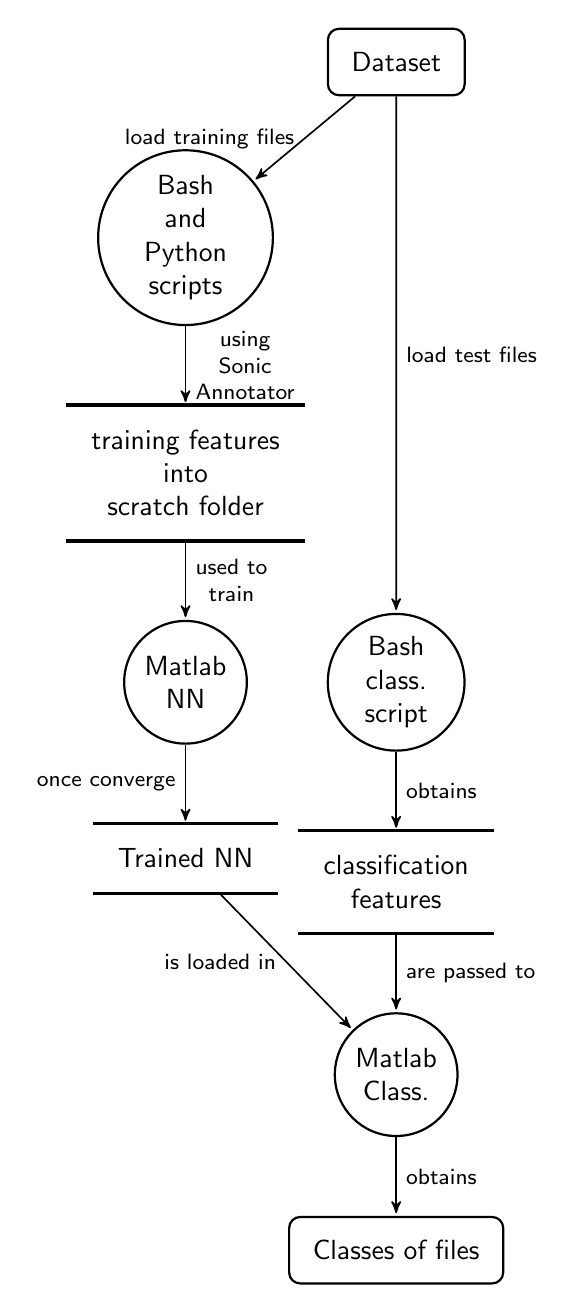
\begin{tikzpicture}[
  font=\sffamily,
  every matrix/.style={ampersand replacement=\&,column sep=2cm,row sep=2cm},
  source/.style={draw,thick,rounded corners,inner sep=.3cm},
  process/.style={draw,thick,circle},
  sink/.style={source},
  datastore/.style={draw,very thick,shape=datastore,inner sep=.3cm},
  dots/.style={gray,scale=2},
  to/.style={->,>=stealth',shorten >=1pt,semithick,font=\sffamily\footnotesize},
  every node/.style={align=center}]

  % Position the nodes using a matrix layout
    \node[source] (dataset) {Dataset};
      \node[process, below left = of dataset] (bps) {Bash\\and\\Python\\scripts};
      \node[datastore, below = of bps] (Tfeatures) {training features\\into\\scratch folder};
      \node[process, below = of Tfeatures] (NN) {Matlab\\NN};
      \node[datastore, below = of NN] (trained_nn) {Trained NN};
      \node[process, right = of NN] (bcs) {Bash\\class.\\script};
      \node[datastore, below = of bcs] (Cfeatures) {classification\\features};
      \node[process, below = of Cfeatures] (mat_class) {Matlab\\Class.};
      \node[sink, below = of mat_class] (classification) {Classes of files};


  % Draw the arrows between the nodes and label them.
  \draw[to] (dataset) -- node[midway,left] {load training files} (bps);
  \draw[to] (bps) -- node[midway,right] {using\\Sonic\\Annotator} (Tfeatures);
  \draw[to] (Tfeatures) -- node[midway,right] {used to\\train} (NN);
  \draw[to] (NN) -- node[midway,left] {once converge} (trained_nn);
  \draw[to] (dataset) -- node[midway,right] {load test files} (bcs);
  \draw[to] (trained_nn) -- node[midway,left] {is loaded in} (mat_class);
  \draw[to] (bcs) -- node[midway,right] {obtains} (Cfeatures);
  \draw[to] (Cfeatures) -- node[midway,right] {are passed to} (mat_class);
  \draw[to] (mat_class) -- node[midway,right] {obtains} (classification);
\end{tikzpicture}
\caption{Workflow of the proposed system}\label{fig:workflow}
\end{center}
\end{figure}

\section{Acknowledgements}\label{sec:acknowledgements}
This research has been developed as a Master's degree final project at the Department of Computer Systems and Computation of the Polytechnic University of Valencia.

 

\begin{thebibliography}{citations}

\bibitem{pan14id} 
Efstathios Stamatatos, Walter Daelemans, Ben Verhoeven, Martin Potthast, Benno Stein, Patrick Juola, Miguel A. Sanchez-Perez and Alberto Barrón-Cedeño:
``Overview of the Author Identification Task at PAN 2014'',
{\it Bauhaus-Universität Weimar}, 
pp.~10--16, 2014.

\bibitem{pan13pr} 

Francisco Rangel, Paolo Rosso, Moshe Koppel, Efstathios Stamatatos, Giacomo Inches:
``Overview of the Author Profiling Task at PAN 2013'',
{\it Bauhaus-Universität Weimar}, 
pp.~6--10, 2014.

\bibitem{mirex14res}
J. Stephen Downie and IMIRSEL:
``MIREX 2014 Evaluation Results'',
{\it University of Illinois at Urbana-Champaign}

\bibitem{sonic_visualizer}
Chris Cannam, Christian Landone, and Mark Sandler:
``Sonic Visualiser: An Open Source Application for Viewing, Analysing, and Annotating Music Audio Files'',
{\it Proceedings of the ACM Multimedia},
2010 International Conference

\bibitem{sonic_annotator}
Chris Cannam, Michael O. Jewell, Christophe Rhodes, Mark Sandler, and Mark d'Inverno:
``Linked Data and You: Bringing music research software into the Semantic Web'',
{\it Journal of New Music Research},
Volume 39, no.~4, pp.~313--325, 2010

\bibitem{rasmusen}
Rasmus Berg Palm:
``Prediction as a candidate for learning deep hierarchical models of data'',
{\it Technical University of Denmark, DTU Informatics},
2012

\bibitem{desportes}
Yvonne Desportes and Alain Bernaud:
``Manuel pratique pour l'approche des styles, de Bach à Ravel'',
{\it Conservatoire National Supérieur de Paris},
1979

\end{thebibliography}


\end{document}
